\chapter{Testing Process}
\label{cha:testing_process}

\section{Introduction}
\label{sec:testing_process_intro}
The testing process for the Library Management System is a structured and multi-layered approach designed to ensure the delivery of a high-quality, reliable, and robust application. Its primary goal is to systematically verify and validate that the system meets the functional and non-functional requirements detailed in the Software Requirements Specification (SRS). This process is integral to mitigating risks, identifying defects early in the development lifecycle, and ultimately ensuring user satisfaction.

Our methodology emphasizes automation to facilitate a continuous integration and testing pipeline. By leveraging containerization with Docker, we establish consistent and isolated environments for development, testing, and production. This is crucial for achieving reliable and reproducible test outcomes, eliminating the "it works on my machine" problem. This chapter details the entire process, from the setup of the test environment to the execution of various testing levels and the management of defects. A visual representation of our high-level automated testing process is shown in Figure \ref{fig:testing_process_flowchart}.

\begin{figure}[H]
    \centering
    \resizebox{0.8\textwidth}{!}{%
    \begin{tikzpicture}[
        node distance=1.5cm and 1cm,
        block/.style={rectangle, draw, fill=blue!10, text width=8em, text centered, rounded corners, minimum height=2.5em, drop shadow},
        line/.style={draw, -{Stealth[length=2mm]}},
        cloud/.style={ellipse, draw, fill=gray!10, minimum height=1.8em, drop shadow}
    ]
        % Nodes
        \node[block] (commit) {Developer Commits Code to Git};
        \node[block, below=of commit] (ci_trigger) {CI Pipeline Triggered (e.g., on Git Push)};
        \node[block, below=of ci_trigger, text width=10em] (build) {Build Docker Images \& Start Containers (\texttt{docker-compose -f docker-compose.test.yml up})};
        \node[block, below left=of build] (unit_integration) {Run Backend Unit \& Integration Tests (Jest/Supertest)};
        \node[block, below right=of build] (component) {Run Frontend Component \& Unit Tests (React Testing Library)};
        \node[block, below=of build, yshift=-3cm, text width=10em] (e2e) {Run End-to-End Tests (Cypress)};
        \node[block, below=of e2e] (report) {Generate \& Archive Test Reports (Jest HTML \& Cypress Videos/Screenshots)};
        \node[cloud, below=of report, text width=7em] (review) {Team Reviews Results \& Manages Defects};

        % Paths
        \path [line] (commit) -- (ci_trigger);
        \path [line] (ci_trigger) -- (build);
        \path [line] (build) -- (unit_integration);
        \path [line] (build) -- (component);
        \path [line] (unit_integration) -- (e2e);
        \path [line] (component) -- (e2e);
        \path [line] (e2e) -- (report);
        \path [line] (report) -- (review);
        \path [line, dashed] (review.west) -| ++(-2,0) |- (commit.west);
    \end{tikzpicture}
    }
    \caption{High-Level Automated Testing Process Flowchart}
    \label{fig:testing_process_flowchart}
\end{figure}


\section{Test Environment and Configuration}
\label{sec:test_environment}
A consistent and reproducible test environment is the cornerstone of our testing strategy. We use Docker and Docker Compose to define and manage the application stack, ensuring that tests are executed in an environment that mirrors production as closely as possible. This minimizes environment-specific defects and guarantees that a test that passes on one developer's machine will also pass in the CI pipeline.

The entire test environment is orchestrated by the \texttt{docker-compose.test.yml} file and configured via the \texttt{.env.test} file. This setup allows any team member to spin up the full test stack with a single command (\texttt{docker-compose -f docker-compose.test.yml up --build}). The services defined are:
\begin{itemize}[noitemsep]
    \item \texttt{server-test}: The Node.js backend application. For API and integration tests, it is configured via \texttt{.env.test} to connect to an in-memory MongoDB server. This provides significant advantages: test isolation (no data leakage between tests), speed (no disk I/O), and simplicity (no need for manual database cleanup).
    \item \texttt{mongo-test}: The MongoDB database. While most automated tests use the in-memory version, this service is available for specific tests that may require validation against a persistent database instance.
    \item \texttt{client-test}: The React frontend application, serving the user interface against which end-to-end tests are run.
    \item \texttt{cypress-e2e}: A dedicated container that runs the Cypress test runner for executing end-to-end tests against the client and server. It is configured to communicate with the other services within the Docker network.
\end{itemize}

This containerized architecture, illustrated in Figure \ref{fig:docker_test_env}, is paramount for maintaining testing integrity across all development and deployment stages.

\begin{figure}[H]
    \centering
    \resizebox{\textwidth}{!}{%
    \begin{tikzpicture}[
        node distance=2.5cm and 3cm,
        container/.style={
            rectangle, 
            draw, 
            thick, 
            rounded corners, 
            fill=blue!5, 
            minimum height=2.5cm, 
            minimum width=3.5cm,
            text width=3cm, 
            align=center,
            drop shadow
        },
        env_box/.style={
            rectangle, 
            draw, 
            dashed, 
            thick,
            color=gray,
            rounded corners,
            inner sep=1cm
        },
        arrow_label/.style={
            midway,
            fill=white,
            inner sep=1pt,
            font=\footnotesize
        },
        line/.style={draw, -{Stealth[length=3mm]}, thick}
    ]
        % Service Nodes
        \node[container] (cypress) {\textbf{Cypress E2E Container} \\ \texttt{cypress-e2e}};
        \node[container, right=of cypress] (client) {\textbf{React Client Container} \\ \texttt{client-test}};
        \node[container, right=of client] (server) {\textbf{Node.js Server Container} \\ \texttt{server-test}};
        \node[container, right=of server] (mongo) {\textbf{MongoDB Container} \\ \texttt{mongo-test}};
        
        % Environment Bounding Box
        \node[env_box, fit=(cypress) (mongo), label={[yshift=0.4cm]above:\textbf{Docker Network (Orchestrated by \texttt{docker-compose.test.yml})}}] (docker_env) {};

        % Arrows with labels
        \path [line] (cypress) -- (client) node[arrow_label, font=\tiny] {User Interaction};
        \path [line] (client) -- (server) node[arrow_label, font=\tiny] {API Calls (HTTP/S)};
        \path [line] (server) -- (mongo) node[arrow_label, font=\tiny] {DB Queries};
        
        % Internal Test Runner Labels
        \node[below, font=\small\itshape, text width=3cm, align=center, yshift=-1cm] at (client.south) {(Runs React Testing Library / Jest)};
        \node[below, font=\small\itshape, text width=3cm, align=center, yshift=-1cm] at (server.south) {(Runs Jest / Supertest)};

    \end{tikzpicture}
    }
    \caption{Docker-Based Test Environment Architecture}
    \label{fig:docker_test_env}
\end{figure}

\section{Testing Levels and Automation Frameworks}
\label{sec:testing_levels}
Our testing process is composed of several distinct levels, each targeting a different part of the application and utilizing specialized tools and techniques to provide comprehensive coverage.

\subsection{Unit Testing}
\label{subsec:unit_testing}
Unit tests form the foundation of our testing pyramid, focusing on the smallest individual components (units) of the system in isolation.
\begin{itemize}
    \item \textbf{Backend (Server):} We use the \textbf{Jest} framework to test individual controllers, models, and utility functions. Mocks and stubs are used extensively to isolate units from external dependencies. For example, in \texttt{bookController.test.js}, the \texttt{Book} model is mocked to simulate database interactions, ensuring the test validates only the controller's internal logic. Similarly, tests for models themselves (e.g., \texttt{book.test.js}) verify schema validations and default values without needing a database connection.
    
    \item \textbf{Frontend (Client):} We use \textbf{React Testing Library} with Jest to test individual React components and custom hooks. Component tests verify that they render correctly given specific props and that they respond as expected to simulated user interactions. For instance, tests for \texttt{LoginForm.js} check for the presence of input fields and validate that clicking the submit button triggers the correct callback function. We also test utility functions like \texttt{formatTime.js} and \texttt{formatNumber.js} to ensure data is displayed correctly across the UI.
\end{itemize}

\begin{lstlisting}[language=JavaScript, caption={Example of a Backend Unit Test for \texttt{bookController.js}}, label={lst:jest-unit-test}]
// From: server/__tests__/unit/controllers/bookController.test.js

const bookController = require('../../../controllers/bookController');
const Book = require('../../../models/book');

// Mock the Book model to isolate the controller logic
jest.mock('../../../models/book');

describe('Book Controller - getBookById', () => {
    it('should return a book with status 200 if a valid ID is passed', async () => {
        const mockBook = { _id: '60c72b2f9b1d8c001f8e4c6d', title: 'Test Book', author: 'Author Name' };
        Book.findById.mockResolvedValue(mockBook);

        const req = { params: { id: '60c72b2f9b1d8c001f8e4c6d' } };
        const res = {
            status: jest.fn().mockReturnThis(),
            json: jest.fn()
        };

        await bookController.getBookById(req, res);

        expect(res.status).toHaveBeenCalledWith(200);
        expect(res.json).toHaveBeenCalledWith(mockBook);
    });
});
\end{lstlisting}

\subsection{Integration Testing}
\label{subsec:integration_testing}
Integration tests focus on verifying the interactions and data flow between different parts of the system.
\begin{itemize}
    \item \textbf{Backend API Testing:} We use \textbf{Jest} and \textbf{Supertest} to perform integration testing on our API endpoints. These tests are critical for ensuring that controllers, models, and services work together as expected. The tests run against a live server instance connected to an in-memory MongoDB database to ensure a clean state for each test suite. We test not only basic CRUD operations but also complex business workflows. For example, \texttt{borrowal.api.test.js} tests the full lifecycle of borrowing and returning a book, while \texttt{bookReferentialIntegrity.api.test.js} ensures that a book cannot be created with a non-existent author.
    
    \item \textbf{Frontend Component Integration:} At the component level, we test how multiple components collaborate to deliver a piece of functionality. For example, on the \texttt{AuthorPage.jsx}, we test the integration between the main data table, the \texttt{AuthorDialog.jsx} (for adding/editing), and the search/filter toolbar, ensuring that actions performed in one component correctly update the state and rendering of the others.
\end{itemize}

\subsection{System (End-to-End) Testing}
\label{subsec:system_testing}
System testing validates the complete, integrated application workflow from a user's perspective. We use \textbf{Cypress} for our end-to-end (E2E) tests because of its reliability and powerful debugging features. These tests simulate real user scenarios by interacting with the application through the browser, just as a user would.

Cypress tests cover critical user journeys derived from the use cases in the SRS (Section 7), such as:
\begin{itemize}[noitemsep]
    \item \textbf{UC-001 (User Login):} As shown in \texttt{authentication\_authorization.cy.ts}, a test logs in as an admin and verifies access to the dashboard.
    \item \textbf{UC-002 \& UC-004 (Entity Management):} The \texttt{entity\_management.cy.ts} script simulates an admin creating a new author, then a new genre, and finally a new book that uses the newly created author and genre.
    \item \textbf{UC-003 (Borrow a Book):} The \texttt{full\_lifecycle.cy.ts} test simulates a member logging in, searching for a book, borrowing it, and then viewing it in their borrowal history.
    \item \textbf{Authorization:} Tests also explicitly verify access control rules, such as ensuring a non-admin user receives a "403 Forbidden" or is redirected when attempting to access administrative API endpoints or frontend routes.
\end{itemize}
To manage test data, Cypress uses fixtures (e.g., \texttt{user-data.json}) to provide consistent user credentials and other data inputs for the tests.

\begin{lstlisting}[language=JavaScript, caption={Example of a Cypress E2E Test for User Login}, label={lst:cypress-e2e-test}]
// From: e2e/cypress/e2e/authentication_authorization.cy.ts

describe('Authentication and Authorization', () => {
  it('should allow an admin user to log in and see the main dashboard', () => {
    // Visit the login page
    cy.visit('/login');

    // Use test data from a fixture file
    cy.fixture('user-data.json').then((userData) => {
      cy.get('input[name="email"]').type(userData.adminUser.email);
      cy.get('input[name="password"]').type(userData.adminUser.password);
    });
    
    // Click the submit button
    cy.get('button[type="submit"]').click();

    // Assert that the URL has changed to the dashboard
    cy.url().should('include', '/dashboard/app');
    
    // Assert that a key element of the dashboard is visible to confirm success
    cy.contains('h4', 'Welcome back').should('be.visible');
  });
});
\end{lstlisting}

\section{Test Execution and Reporting}
\label{sec:test_execution_reporting}
Test execution is streamlined and automated through npm scripts defined in the respective \texttt{package.json} files, enabling easy execution both locally and in a CI/CD pipeline.
\begin{itemize}
    \item \textbf{Backend Tests:} Running \texttt{npm test} in the \texttt{/server} directory executes all Jest-based unit and integration tests.
    \item \textbf{Frontend Tests:} Running \texttt{npm test} in the \texttt{/client} directory executes all React Testing Library component tests.
    \item \textbf{E2E Tests:} Running \texttt{npm run cypress:run} in the \texttt{/e2e} directory executes the full suite of Cypress end-to-end tests in headless mode.
\end{itemize}

Upon completion, the test frameworks generate detailed reports. Jest is configured with \texttt{jest-html-reporters} to produce a comprehensive HTML report (located in \texttt{server/test-report/}), which provides a shareable overview of test suite results, pass/fail status, execution times, and code coverage metrics. Code coverage is particularly important as it helps the team identify areas of the application that are not covered by tests. Cypress automatically generates video recordings of each test run and detailed screenshots upon failure, which are invaluable for quickly diagnosing the root cause of an issue.

\begin{figure}[H]
    \centering
    % Placeholder for a test report screenshot
    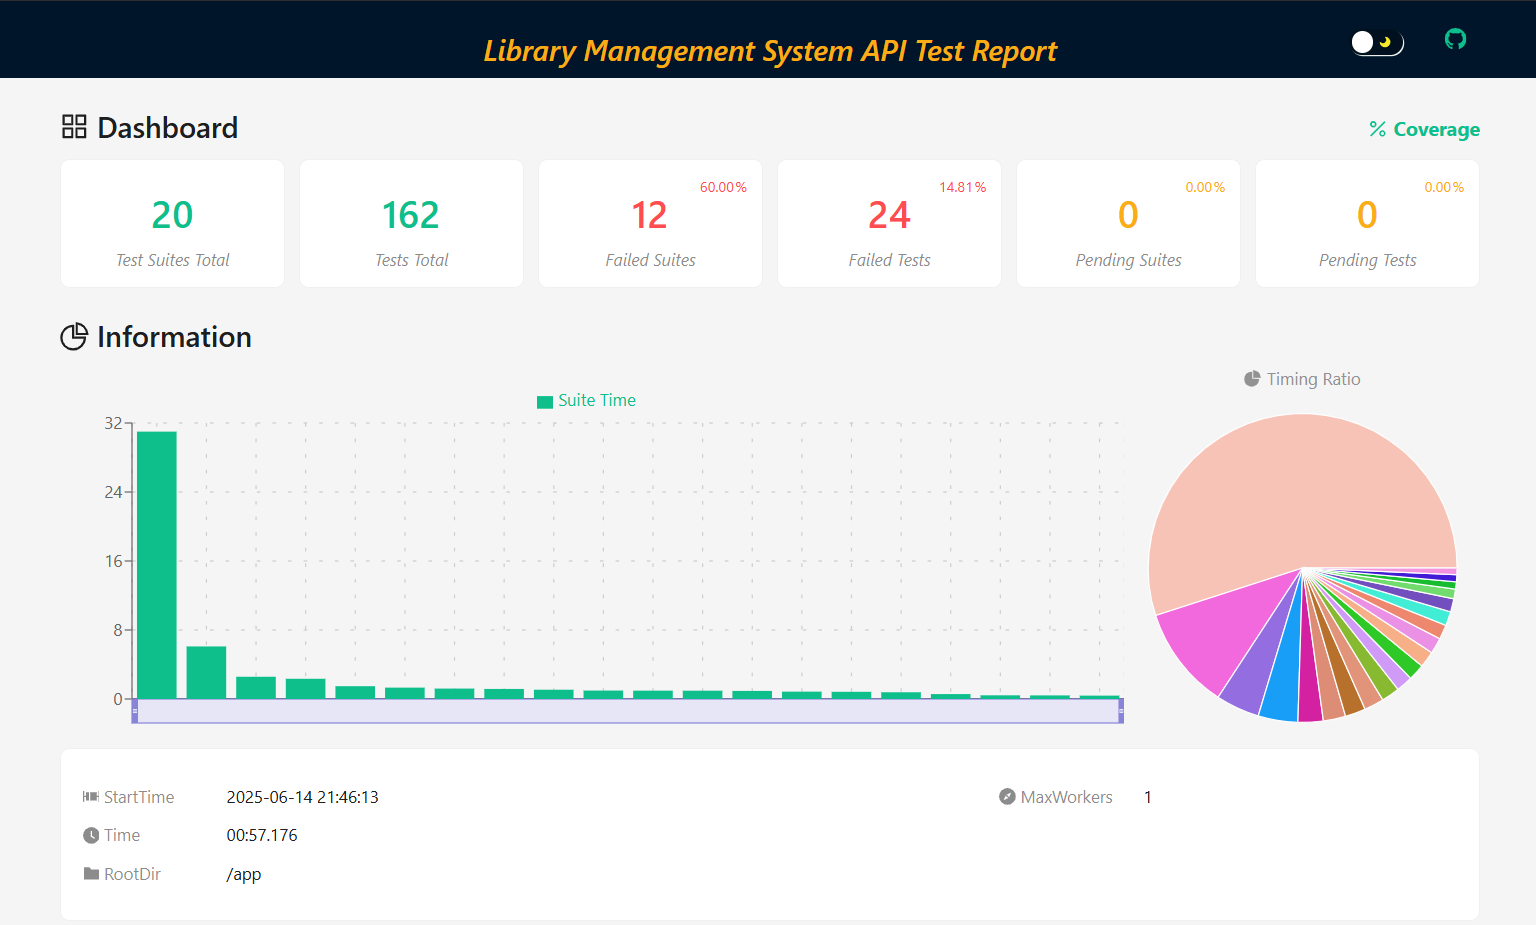
\includegraphics[width=\textwidth]{assets/jest/jest_report_screenshot.png}
    \caption{Example of an HTML Test Report from Jest}
    \label{fig:test_report_example}
\end{figure}

\section{Defect Management}
\label{sec:defect_management}
A formal defect management process is essential for tracking and resolving issues discovered during testing. Our process ensures that no bug is lost and that every issue is triaged, prioritized, and resolved in a timely manner. While a dedicated tool like Jira or Trello is recommended, this process can also be managed using GitHub Issues.

The defect lifecycle is as follows:
\begin{enumerate}
    \item \textbf{Discovery and Logging:} When a test fails or a bug is found during manual testing, the tester logs a new defect. The defect report includes a clear title, a detailed description of the issue, steps to reproduce it, the expected result vs. the actual result, and any relevant artifacts like screenshots, logs, or video recordings from Cypress.
    \item \textbf{Triage and Prioritization:} The Test Manager and technical lead review new defects to assess their impact and urgency. Defects are assigned a priority (e.g., Critical, High, Medium, Low) based on factors like severity, scope of impact, and risk to the project timeline.
    \item \textbf{Assignment:} The defect is assigned to the appropriate developer for resolution.
    \item \textbf{Resolution:} The developer fixes the bug, commits the code, and marks the defect as "Resolved." The fix should ideally include a new regression test that specifically targets the bug to prevent it from recurring.
    \item \textbf{Verification:} The tester re-runs the failing test in the updated environment to verify that the fix has resolved the issue and has not introduced any new regressions. If the fix is confirmed, the defect is closed. If not, it is reopened and reassigned to the developer.
\end{enumerate}
This structured workflow ensures accountability and provides clear visibility into the health of the application throughout the development process.
